\documentclass[12pt,a4paper]{scrartcl}

%\usepackage{cite}
\usepackage[authoryear]{natbib}
\usepackage{hyperref}
\usepackage{url}
\usepackage{graphicx}
\usepackage{xcolor}
\usepackage{textcomp}
\usepackage{subfig}
\usepackage{amsmath}
\usepackage{enumerate} % http://ctan.org/pkg/enumerate

\definecolor{steelblue}{rgb}{0.36, 0.54, 0.66}

\newcommand{\git}[0]{\href{https://github.com/raim/PBR}{PBR git}}
\newcommand{\ordered}[0]{\textcolor{steelblue}{\textbf{ordered}}}
\newcommand{\obtain}[0]{\textcolor{orange}{\textbf{obtain}}}
\newcommand{\avail}[0]{\textcolor{green}{\textbf{available}}}
\newcommand{\build}[0]{\textcolor{red}{\textbf{build}}}
\newcommand{\code}[0]{\textcolor{blue}{\textbf{code}}}
\newcommand{\hack}[0]{Hack`a'thing}
\newcommand{\gasometer}[0]{\texttt{Gas`o'meter}}
\newcommand{\liqometer}[0]{\texttt{Liq`o'meter}}
\newcommand{\ph}[0]{h{\small$^{-1}$}}
\newcommand{\ox}[0]{O$_2$}
\newcommand{\cox}[0]{CO$_2$}

\parskip 0.3 cm
\parindent 0 cm

\title{Open and Modular Photobioreactor}
\subtitle{Projects.}

\begin{document}
\maketitle
%\scriptsize
\tableofcontents
%\normalsize
\newpage


\section{Resources - Materials, Designs and Ideas}

Please see the
\href{https://wiki.hhu.de/display/QTBP/1st+QTB+PBR+Hack\%60a'thing}{Hack`a'thing
  Wiki} for link lists of DIY bioreactors, DIY lab ware, 3D printer
designs, general DIY websites, and electronics suppy shops.

All code is at the \href{https://github.com/raim/PBR}{github project}.

\begin{figure}[ht]
  \begin{minipage}{.49\textwidth}
    \subfloat[Dougie's Reactor]{
      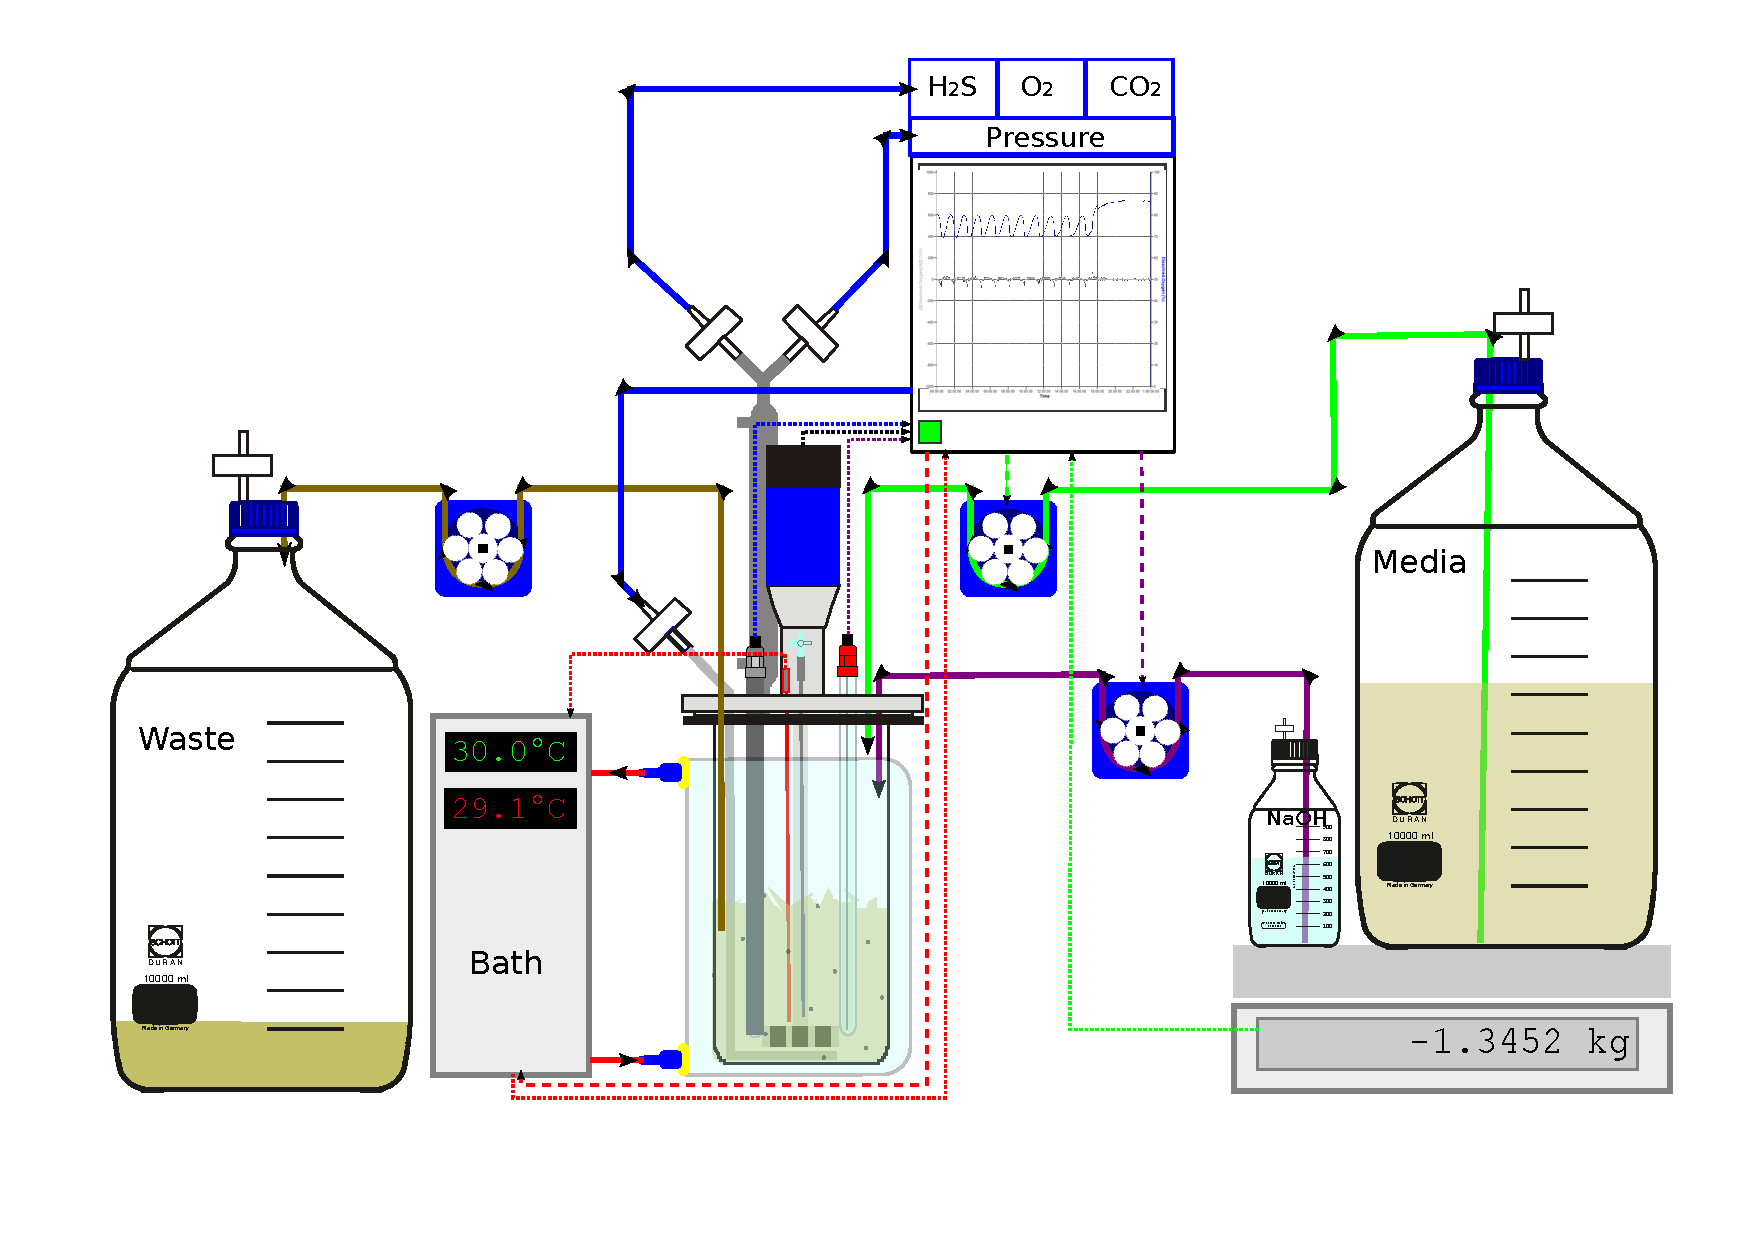
\includegraphics[width=\textwidth]{figures/fermentor_detailed.pdf}\\ 
    }
  \end{minipage}
  \begin{minipage}{.49\textwidth}
    \centering Monod: $\mu = \mu_{max} \frac{S}{S+K_S}$\\
    \subfloat[Snoep \textit{et al.} 2009]{
      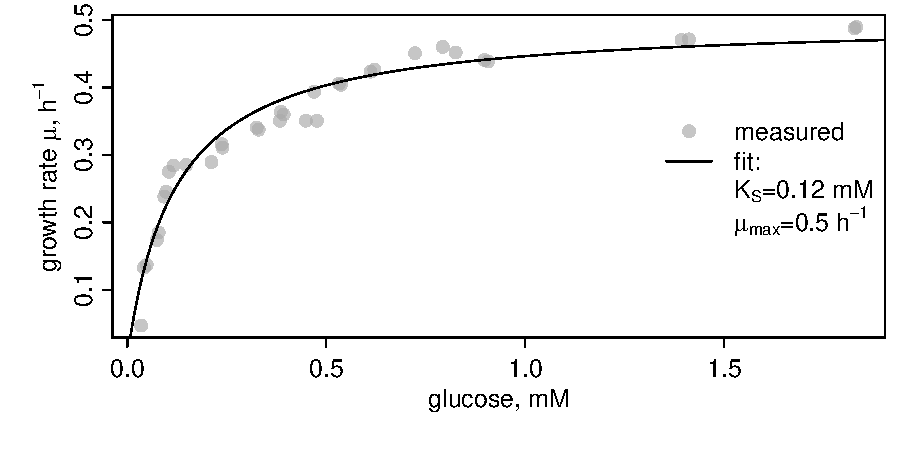
\includegraphics[width=\textwidth]{figures/snoep09_fig2.pdf}
    }
  \end{minipage}
\caption[]{Bioreactors}
\end{figure}

%\vspace{-10ex}

\begin{figure}
\begin{minipage}{.5\textwidth}
  \begin{equation*}
    \label{eqn:ancat}
    \begin{aligned}
      \frac{\text{d}X}{\text{d}t} &= (\mu_{ab} - \phi) X  \\
      \frac{\text{d}S}{\text{d}t} &= \phi (S_{in} - S)-(\mu_{ab} + \mu_{cd}) X\\  
      \frac{\text{d}atp}{\text{d}t} &= (n_{cd} \mu_{cd} - n_{ab} \mu_{ab} - \mu_{m})\frac{C_c}{V_c} - \mu_{ab} atp\\
      \frac{\text{d}G}{\text{d}t} &= k_La (G_{in}^* - G) - n_{g} \mu_{cd} X\\
      adp & = a_{tot} - atp
    \end{aligned}
  \end{equation*}
\end{minipage}
\begin{minipage}{.5\textwidth}
  \begin{equation*}
    \begin{aligned}
      \mu_{ab} &\equiv f(S,atp)\\
      \mu_{cd} &\equiv f(S,G,adp)\\
      \mu_m &\equiv f(S,ROS)
      n_{cd},\,n_{ab} &\equiv f(S) 
    \end{aligned}
  \end{equation*}
\end{minipage}
\caption{Growth in Continuous Culture: liquid and gas flux equations} 
\end{figure}


\newpage
\section{PBR Modules}
\label{proj}

\subsection{Gas Flux: \gasometer{}}
\label{gas}

For measuring gas turnover rates of bio-cultures.
Code in  \texttt{code/gas/gasometer/} at the \git{}.

\paragraph{Project:} 
Run co2meter's
\href{http://www.co2meter.com/collections/co2-sensors/oxygen-sensors}{\ox{}}
and
\href{http://www.co2meter.com/collections/co2-sensors/products/cozir-5-100-co2-sensor}{\cox{}}
sensors via Sainsmart's
\href{http://www.sainsmart.com/featured-products/sainsmart-mega2560-board-3-5-tft-lcd-module-display-shield-kit-for-atmel-atmega-avr-16au-atmega8u2.html}{Arduino
  Mega+Touch screen}); add a digital mass flow meter
\href{http://www.aalborg.com/index.php/main_page/product_overview/id_product_overview/63}{Aalborg
  XFM}; write calibration routines for all sensors; build water trap
and tubing to connect to the PSI or our DIY reactor and increase gas
transfer (smaller bubbles) and decrease overall gas flow so that we
can measure cellular activity. Perhaps add valve control to measure
multiple reactors in series.

\begin{enumerate}
\item \build{}: COZIR and UV Flux probes to Arduino Mega's Tx/Rx pins,
  solder 5V/3.3V and Gnd connections to touchscreen shield; \code{}:
  display of measurement values on screen, and optional ``record
  data'' mode to store data on the SD card of the touchscreen
\item \build{} water trap, tubing path from reactor, and casing for
  sensors and Arduino; \build{} improved gassing system (glas
  blowers!) to allow lower flow
\item \code{} sensor calibration routines via touch-screen (use PSI
  gas mixing system)
\item \build{} \& \code{} interface to Aalborg XFM digital mass flow
  meter: connect the Aalborg's RS 485 interface to Arduino hardware
  serial Tx3/Rx3, and Ground
\item \build{} \& \code{} valve control to measure several reactors;
  connect via Arduino software serial connections; perhaps attach to
  PSI Multicultivator
\end{enumerate}

\paragraph{Resources:}
\begin{itemize}
\item Sensor manuals in \texttt{manuals/offgas/} at the
  \git{}:\\
  \texttt{Manual-CM-0201-UV-Flux-Oxygen.pdf},
  \texttt{Manual-GSS-Sensors.pdf}, and\\
  \texttt{A\_XFM\_Manual\_TD0701M[...].pdf}
\end{itemize}

\paragraph{Materials:}

\begin{itemize}
\item Sainsmart's Arduino Mega R3 + 3.2' Touchscreen 
\item co2meter's \cox{} and \ox{} sensors, with cap adapter for flow:
  \href{http://www.co2meter.com/collections/co2-sensors/products/cozir-5-100-co2-sensor}{COZIR} and \href{http://www.co2meter.com/collections/co2-sensors/products/uv-flux-oxygen-sensor}{UV Flux}
\item Aalborg XFM, with RS 485 interface + Arduino TTL-to-RS485 converter
\item Temperature \& Humidity sensor: AM2302 \href{http://www.elecrow.com/temperature-humidity-sensor-proam2302-p-513.html}{via elecrow}
\item Valve system for gas tubing, controllable \textit{via} serial
  interface
\end{itemize}

\begin{figure}[ht]
  \begin{minipage}{.49\textwidth}
    \subfloat[The Gas`o'meter: making of]{
      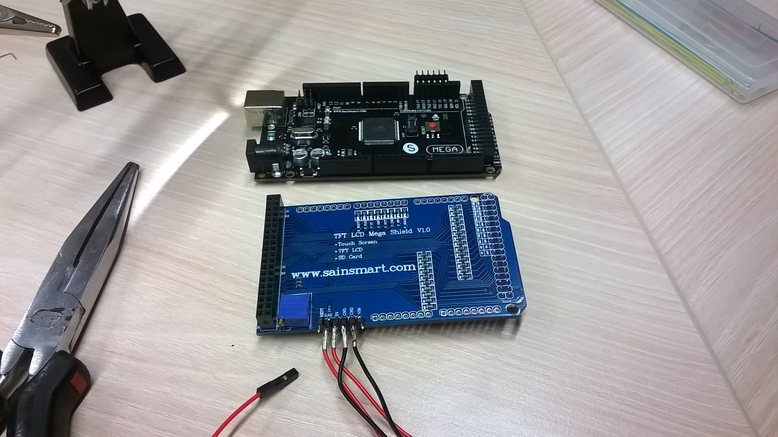
\includegraphics[width=\textwidth]{figures/offgas_makingof1.png}
    }
  \end{minipage}
  \begin{minipage}{.49\textwidth}
    \subfloat[The Gas`o'meter: making of]{
      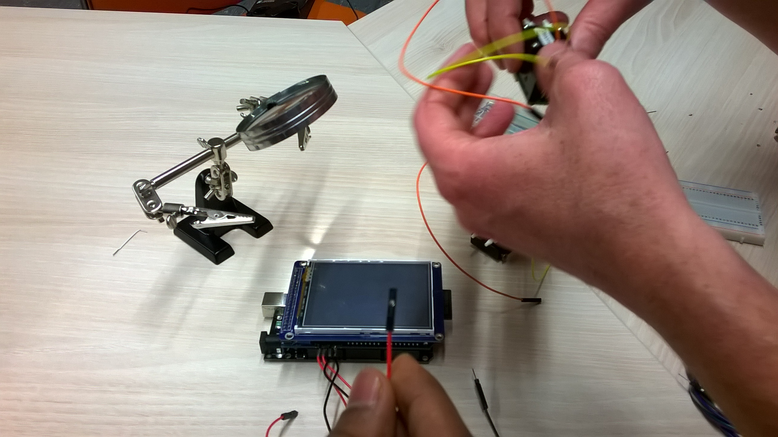
\includegraphics[width=\textwidth]{figures/offgas_makingof2.png}
    }
  \end{minipage}

  \begin{minipage}{.49\textwidth}
    \subfloat[The Gas`o'meter]{
      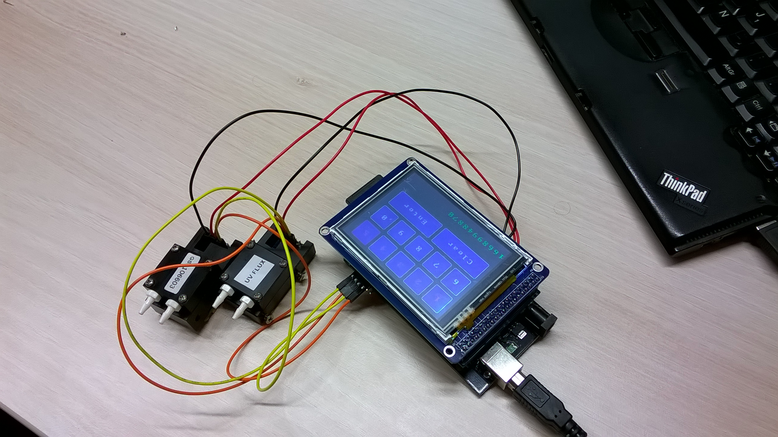
\includegraphics[width=\textwidth]{figures/offgas_makingof3.png}
    }
  \end{minipage}
  \begin{minipage}{.49\textwidth}
    \subfloat[Room 03.30, 2016-01-13]{
      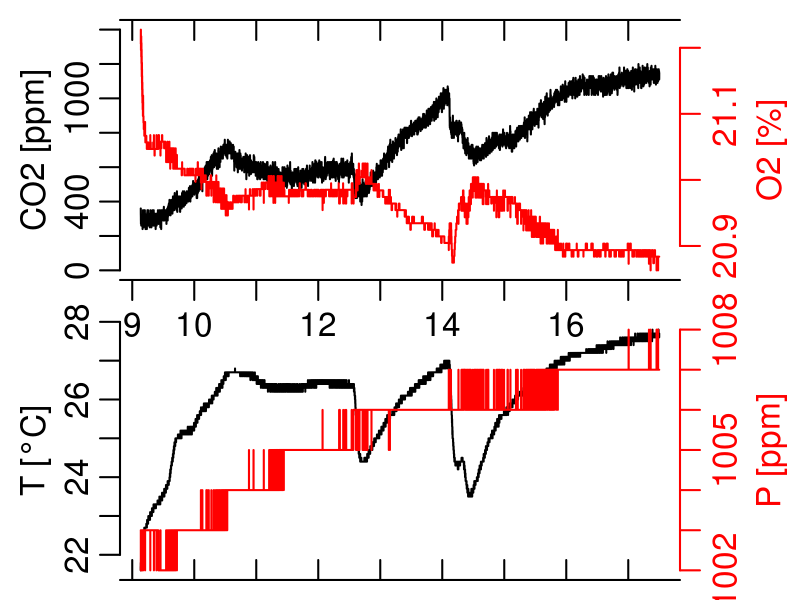
\includegraphics[width=\textwidth]{figures/20160113.png}
    }
  \end{minipage}
\caption[]{\textbf{Gas Measurement Module.}}
\end{figure}

\newpage
\subsection{Liquid Flux: \liqometer{}} 
\label{cult}

For running cultures in chemostat (continuous culture) or turbidostat modes. 
Code in  \texttt{code/liquid/} at the \git{}.

\paragraph{Project:} build a module consisting of media and waste bottles, 
a reactor vessel, peristaltic pump(s), and a scale; pump and scale are
controlled \textit{via} serial interfaces from an
Arduino+Touchscreen. The flow rate is controlled \textit{via} the pump
motor speed and recorded \textit{via} the scale; the flow rate is
recorded or can be set after a setup-specific (tubing) calibration
routine


\begin{enumerate}
\item \build{} a simple reactor vessel (Schott bottles) with liquid
  media flow, from media bottles through reactor vessel and out to
  waste bottle 
\item \code{}: calibration routine for the weight sensor module
\item \code{}: analog control of peristaltic motor speed and recording of
  weight loss and/or gain to record mass flow (g/min)
\item \code{}: routine to calibrate pump speed to weight loss/gain
  for a specific setup; store calibration on SD card, which allows
  to also set pump speed in g/min, or if provided with a culture
  volume, as culture dilution rate (\ph{})
\item \build{} \& \code{}: combine with \ref{spec} to make
  turbidostatic control
\item \build{}: add gassing system of project \ref{gas} to make a first
  simple bioreactor
\end{enumerate}

\paragraph{Resources:}
\begin{itemize}
\item \href{ https://github.com/bogde/HX711}{Arduino library for Elecrow weight sensor kit} based on \href{https://github.com/aguegu/ardulibs/tree/master/hx711}{older version}
\item \href{https://cdn.sparkfun.com/datasheets/Sensors/ForceFlex/hx711_english.pdf}{HX711 24-bit analog-to-digital converter (ADC) for load cells}
\end{itemize}

\paragraph{Materials:}
\begin{itemize}
\item Sainsmart's Arduino Mega R3 + 3.2' Touchscreen + Arduino Motor Shield R3
\item Scale:\\ Elecrow Weight Sensor kit 3kg for Arduino
  \href{http://www.elecrow.com/weight-sensor-kit-3kg-p-883.html}{via
    elecrow}
\item Peristaltic pumps, options:\\
  12V DC motor (5000 rpm): \href{http://www.ebay.de/itm/2stk-12V-Schlauchpumpe-Dosierpumpe-Peristaltikpumpe-Wasser-Pumpe-Silikonschlauch-/191363832760}{at ebay}\\
  12V/24V stepper motor and metal tube holder (pump head) \href{http://de.aliexpress.com/item/Peristaltic-Pump-with-step-motor-precision-peristaltic-pump-peristaltic-filling/2013487841.html}{via aliexpress}\\
  12V Nema17 stepper motor with 3D-printed pump head
\end{itemize}

\begin{figure}[ht]
  \begin{minipage}{.49\textwidth}
    \subfloat[Elecrow Scale Module, 3 kg]{
      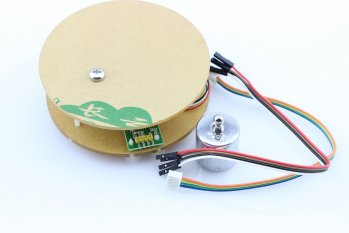
\includegraphics[width=.8\textwidth]{figures/elecrow_scale.png}
    }\\
    \subfloat[Adafruit Peristaltic Pump]{
      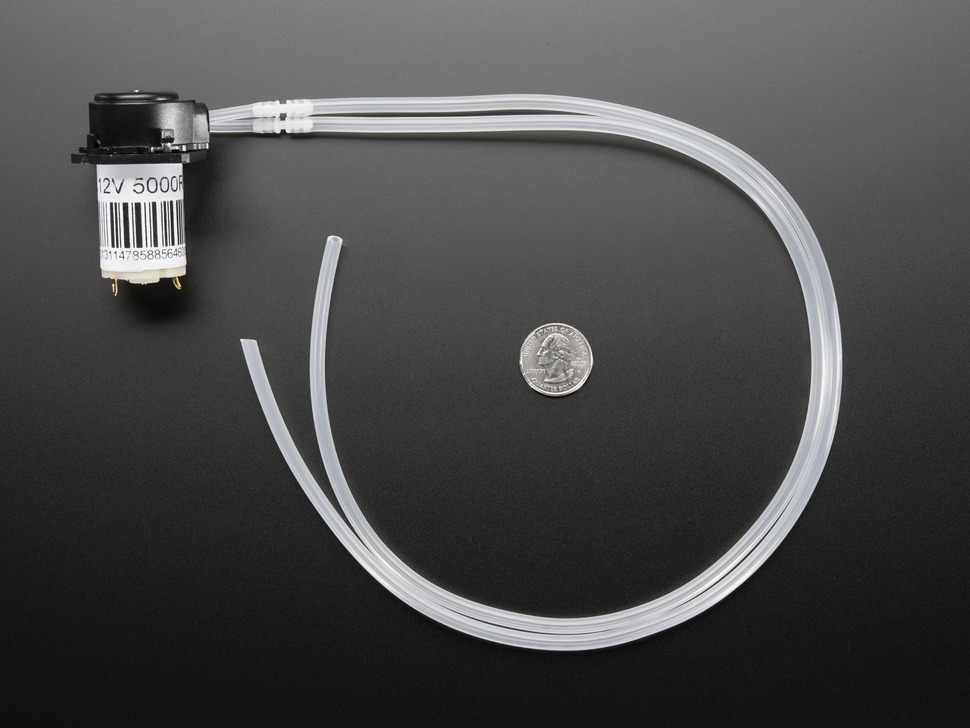
\includegraphics[width=.8\textwidth]{figures/adafruit_pump.png}
    }
  \end{minipage}
  \begin{minipage}{.5\textwidth}
    \subfloat[Fritzing scheme for the Pump]{
      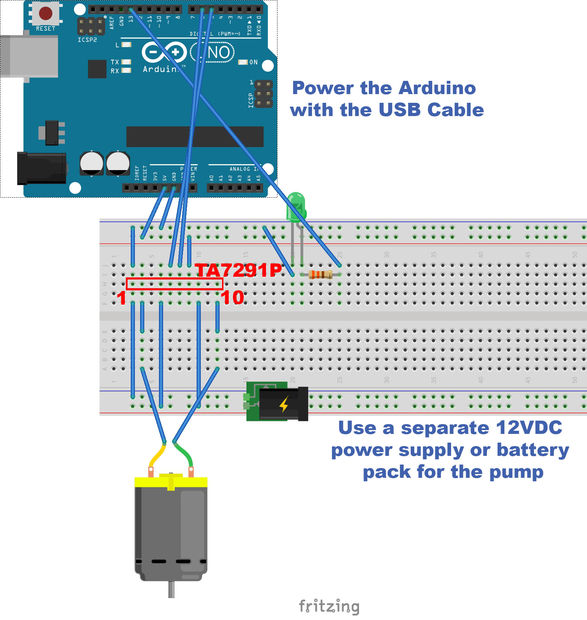
\includegraphics[width=\textwidth]{figures/pump_fritzing.png}
    }
  \end{minipage}
\caption[]{\textbf{Continuous Culture Module}. The elecrow scale
  module is based on the HX711 load-cell amplifier (24-bit analog-
  to-digital converter) and connected to 5V, Gnd and two analog pins
  of the Arduino and comes with an
  \href{http://www.elecrow.com/wiki/index.php?title=Weight_Sensor_Scales_Kit-_20KG}{Arduino
    library}. An \href{https://www.adafruit.com/product/1150}{Adafruit
    peristaltic pump} (12V; a ``geared down DC motor'') is run via
  the Arduino motor shield or alternatively via a a Toshiba TA7291P
  Bridge Driver (0-20V 1A; 2A peak)
  (\href{http://www.instructables.com/id/Control-peristaltic-pump-with-TA7291P-and-an-Ardui/}{instructable
    here}). }
\end{figure}

\clearpage
\subsection{Light Flux}
\subsubsection{Light Scatter for Biomass} 
\label{scatter}

\paragraph{Background.}
This technique is known as nephelometry.  Light scatter can be used as
an estimate of cell number and biomass, and gives a monotonous signal
for OD$>1$ without dilution \citep{Hancher1974}. This would allow use
as an online measurement tool, either in a flow-cell, where culture is
pumped through \citep{Hancher1974}, or directly through glass wall of
culture vessels. Back-scatter, at 180\textdegree{}, can be used to
measure from the outside of a transpartent reactor vessel
\citep{Ude2014, Bruder2016}. Measurement of scatter at 90\textdegree{}
works better for low to intermediate cell densities \citep{Ude2014}.

A problem is that scatter can not be blanked to empty medium, and the
value will depend on the light intensity and path, etc. A solution
would be to express the measured value as a fraction of a standard
scattering solution. Possible standards are discussed by
\cite{Buffone1976}. The commercial solution Ludox has been used by
\cite{Maron1954} and may be standardized enough for such a purpose,
e.g. \href{http://www.sigmaaldrich.com/catalog/product/aldrich/420786}{Sigma Aldrich, CAS Number 7631-86-9, LUDOX\textsuperscript{\textregistered} TM-40 colloidal silica}.

\paragraph{Preliminary Results.}
We found a linear relation of 90\textdegree{} scatter for OD 1--12 for
\textit{E. coli}, at ca. 640 nm the peak of a red light LED.\\
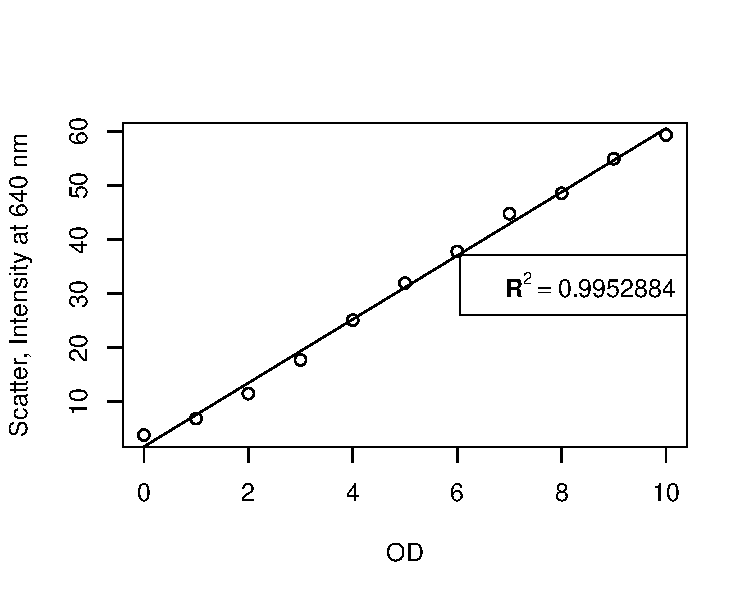
\includegraphics[width=.4\textwidth]{../data/scatter_test1.pdf}

\paragraph{Ressources:}
\begin{itemize}
  \setlength\itemsep{0em}
\item DIY Arduino-based Modules:
  \begin{itemize}
    \setlength\itemsep{-1em}
  \item \url{https://github.com/ebgoldstein/OpenOBS} is a simple
    backscatter sensor with LED display, 
  \item \url{https://hackaday.io/project/12125-pulse-profiling-underwater-light-sensor}
    is a more involved underwater light- and backscatter sensors
  \end{itemize}
\item Commercial Products:
  \begin{itemize}
    \setlength\itemsep{-1em}
  \item \cite{Ude2014} test a shake flask system for PreSens
  \item \cite{Bruder2016} test a shake flask system for Aquila Biolabs
  \end{itemize}
\end{itemize}

\clearpage
\subsubsection{Microplate Illumination} 
\label{led}

\paragraph{Project:} LED illumination for algal growth in microtiter plates for
growth and measurement in a plate reader; with programmable
time-courese of illumination (24 h cycles). An arduino accelerometer
could sense a strong shaking pulse as a signal to stop illumination
for measurements. See for LED intensity setting \href{
  https://www.arduino.cc/en/Tutorial/Fade}{Fade tutorial}, or
\href{https://www.youtube.com/watch?v=PNQ8R1Ptvs4}{video tutorial} for
WS2812 RGB LEDs.

Similar set-ups:
\begin{itemize}
\item microplate illumination platform by the Rust lab: \cite{Lambert2016,Leypunskiy2017} 
\item Light-Plate Apparatus: \cite{Gerhardt2016}
\end{itemize}

Resources:
\begin{itemize}
\item Accelerometer: Adafruit MMA8451
\item LEDs, RGB (WS2812) or just \href{http://www.produktinfo.conrad.com/datenblaetter/175000-199999/180105-da-01-en-LED_0805_TYP_KP_2012SRC_PRV.pdf}{Red LEDs}, ca. 10 Candela
\item Arduino Nano
\item Battery?
\end{itemize}


\clearpage
\subsubsection{Spectrometer} 
\label{spec}
\paragraph{Project:} 
Simple spectrometric measuring tool based on
\href{http://www.avantes.com/products/spectrometers/compactline/item/723-avaspec-mini}{AvaSpec-Mini2048l-V25}

\begin{enumerate}
\item Basic: Connect to Rasperry Pi, using drivers provides by
  Avantes; \code{} simple interface with display and/or recording
  functions
\item Advanced: use LED for absorbance, reflectance, or fluorescence
  measurements; \build{} light paths and perhaps a reactor probe for
  online recording
\end{enumerate}


\paragraph{Resources:}
\begin{itemize}
\item
  \href{http://www.avantes.com/images/productsheets/AvaSpec_Mini5.pdf}{AvaSpec-Mini
    data sheet} in \texttt{manuals/light/} at the \git{}
\item \href{http://www.avantes.com/products/oem/item/220-oem-spectrometers-as5216-microprocessor-board}{The AS5216 microprocessor board} - lib for Rasp. Pi 1 B+ at \texttt{code/light/}
\item \href{http://www.ncbi.nlm.nih.gov/pmc/articles/PMC4641590/}{Tsuda
    \textit{et al.} PLoS ONE 2015}: 3D printed casing for OD measurement
\end{itemize}

\paragraph{Materials:}
\begin{itemize}
\item AvaSpec-Mini2048l-V25, Minispectrometer:\\ Mini
  spectrometer, 2048 Large pixels, grating-MN0600-0.50 (350-885nm),
  OSC, 25\textmu{}m slit, USB2 interface, AvaSoft-Basic
\item Fiber optic cables, VIS/NIR: 1 m, 200 \textmu{}m VIS/NIR and 1m,
  600 \textmu{}m
  SMA terminations, metal protection sleeves
\item Raspberry Pi Version 1 Model B+ or Version 2 (libs for both available) 
\item LED system: use PSI LEDs or \obtain{}
\item Reactor probe: \build{}; 3D print and/or fine mechanics and glas
  blowers
\end{itemize}

\begin{figure}[ht]
  \begin{minipage}{.49\textwidth}
    \subfloat[AvaSpec-Mini 2048]{
      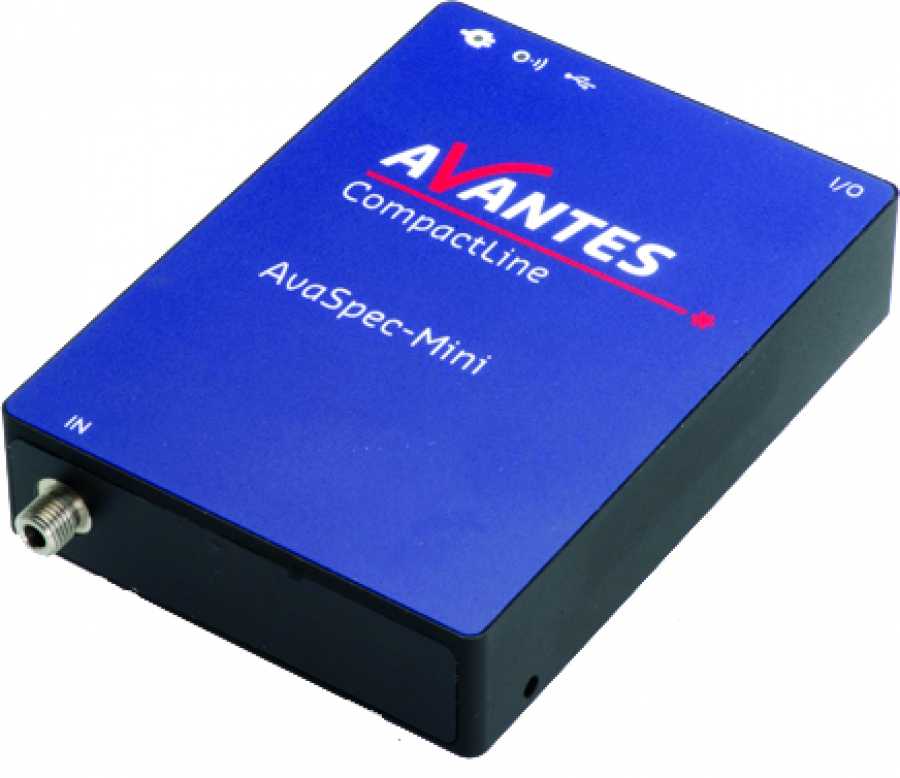
\includegraphics[width=.7\textwidth]{figures/avaspec-mini.png}
    }
  \end{minipage}
  \begin{minipage}{.49\textwidth}
    \subfloat[]{
      \centering setup sketch here
    }
  \end{minipage}
\caption[]{\textbf{Spectrometer Module.}}
\end{figure}


\clearpage
\subsection{The Server}
\paragraph{Project:} a master software running on a (detachable) linux 
desktop that synchronizes and speaks via a comon interface to all
Arduino and Raspberry Pi modules; the modules themselves can interpret
get, set and act impulses (use arguments only when absolutely
necessary).\\ During an initializiation the server may inquire what an
attached module provides (\textit{via} data IDs and SI units,
meaningful time resolution) and handle it automatically. \\ Variable
higher order control or processing logics can be built using defined
data and control IDs. Ultimately, a direct integration with
mathematical models may be desirable.  For example, measured \ox{} and
\cox{} levels may be used to estimate metabolic activities, such as
catabolic ATP/ADP turnover; required data and equations can be loaded
and interpreted \textit{via} SBML encoded models.
\begin{enumerate}
\item \build{} combine of gas (\ref{gas}), liquid (\ref{cult})
  and light (\ref{spec}) modules into a bioreactor
\item \code{}: master program to synchronize and record data from
  the three modules
\item \code{}: combine e.g. \ref{spec} \& \ref{cult} to implement
  turbidostat control
\item \code{}: higher order data evaluation logics, \textit{eg.}, estimate
  metabolic rates from gas exchange measurements
\end{enumerate}


\paragraph{Materials:}
\begin{itemize}
\item \texttt{setTime(time\_t $t$)}: sets the current master time to
  all modules
\item \texttt{get(..., time\_t $t$)}: get all values, currently
  available (with a time stamp), or from a previous time $t$
%\item \texttt{set(..., time\_t $t$)}: sets specific values, now or at an
%  indicated future time $t$
\item \texttt{act(..., time\_t $t$)}: act (switch on and off, set to a
  specific value), now or at future time $t$
\end{itemize}

\newpage
\subsection{Heat Flux: Water Bath Thermostat}
\label{heat}

\paragraph{Project:} build a water bath for growth vessels, control
T, read-out energy required for maintaining constant T and estimate
the amount of heat withdrawn or administered

\begin{enumerate}
\item
\end{enumerate}

\paragraph{Materials:}
\begin{itemize}
\item Jacketed reactor vessel: \build{} or \obtain{}
\item Julabo water bath,
e.g. \href{http://www.laborhandel24.de/9162625-de?utm_source=google_shopping&gclid=Cj0KEQiA496zBRDoi5OY3p2xmaUBEiQArLNnK6uWkryhjvkNdmRLgcg2W_HIO9W1aKaKCO9gmvlkt_MaAmhe8P8HAQ}{F25-ME}
\item Arduino and/or Raspberry Pi
\end{itemize}

\newpage
\subsection{The \texttt{Kaiten Eppi}: Automated Sampling Device} 
\label{sampling}
\paragraph{Projects:} build sterile and automated sampling device; using
a controllable syringe pump, sampling into the \texttt{Kaiten Eppi}
(automated: pump sample into tubes, potentially pre-filled with
chemicals, vortex, and transport them into liquid N$_2$ or other
storage containers)

\paragraph{Materials:}
\begin{itemize}
\item Sainsmart's Arduino Mega \& Touchscreen
\item Sterile sampling device by HHU glas blowers
\item 12V Nema17 Stepper Motor 45oz,0.4A,34mm for 3D printer CE (as in ultimaker2):\\
  \href{http://www.ebay.com/itm/251604407772?_trksid=p2055119.m1438.l2649&ssPageName=STRK\%3AMEBIDX\%3AIT}{via act motor}
\item Plastic syringe pump + 3D-printed holder for pump and motor
\item \texttt{Kaiten Eppi}: \build{} a circular tube-holder, run by a
  stepper motor (same as above for pump)
\end{itemize}


\newpage
\subsection{Single Cell Biology: Microfluidic Device} 
\label{micro}

\paragraph{Project:} Basic microfluidics and live-cell imaging device;
scratch growth chambers and liquid flow channels into microscope slide;
attach 2--3 pumps; and control \textit{via} arduino/screen

\paragraph{Resources:}
\begin{itemize}
\item \href{http://www.ncbi.nlm.nih.gov/pmc/articles/PMC4641590/}{Tsuda \textit{et al.} PLoS ONE 2015: 3D Printed 'Plug and Play' Millifluidic}
\end{itemize}

\paragraph{Materials:}
\begin{itemize}
\item Ilka's lab microscope: \avail{}
\item Microscopy slides: \avail{}
\item 2--3 peristaltic pumps for microfluidics: \obtain{}
\item Sainsmart's Arduino Mega + Touchscreen: \obtain{}
\end{itemize}


\clearpage
%% for new refs: reset to global tata.bib, run latex/bibtex,
%% and use `bibexport -o projects.bib projects.aux`
\bibliographystyle{plainnat}
%\bibliography{/home/raim/ref/tata}
\bibliography{projects}


\end{document}
